\newpage
\section{Reproducible Test Environment}\label{sec:reproducible-test-environment}

Unless stated otherwise, all referenced implementation artifacts in this section originate from the NSAK repository \cite{nsakRepository2026}.

The scope of this thesis is confined to the \gls{AI} based reconnaissance and optionally,
the intrusion detection scenarios~\ref{subsubsec:milestone-ai-scenarios},
including the design and implementation of corresponding drills.

To ensure a controlled and safe evaluation of the implementation, a simulated test environment has to be established.
This approach prevents unintended interference with production systems and ensures reproducibility during the development and testing phases.

For this exact purpose the~\enquote{Environment}\ref{subsec:environment-concept} resource type was implemented into the \gls{NSAK} framework.
In the predecessor project~\ref{sec:predecessor-project-project-2}, a simplified network topology comprising a client (Alice) and a server (Bob) is used to emulate and analyze a \gls{MITM} scenario.
This environment is described in a \gls{Docker Compose} file, located under:
\path|lib/environments/simple_tcp_client_server/compose.yaml|.

The whole setup can be simulated with the following command:
\mintinline{bash}|nsak environment simulate simple_tcp_client_server mitm|.

...

\todo{Maybe it would make sense to describe this in the project 2 section instead}

While \gls{Docker} or \gls{Podman} provides a general-purpose containerization platform, they abstract away most of the lower levels of the network stack and thus lack the support for modeling network topologies.
In the existing implementation this was partially addressed, by using the~\href{https://docs.docker.com/engine/network/drivers/macvlan/}{macvlan} network driver, to enable level 2 networking.
In contrast, \gls{Containerlab} builds upon \gls{Docker Compose} and optimize its functionalities for networking purposes.

The primary advantages of \gls{Containerlab} are:
\begin{itemize}
	\item It's ability to create a reproducible containerized network topology based on a simple configuration file
	\item Support multiple interfaces nodes which closely resemble real-world network devices (in comparison \gls{Docker} typically operates with a single network interface).
	\item The rapid creation, extension and teardown of complete network environments, ensure that each experiment starts from a clean and controlled state.
\end{itemize}
In summary, while OCI containers serves as the underlying container engine, \gls{Containerlab} provides a higher-level network simulation.

Listing~\ref{lst:containerlab-topology-yaml-exampel} in the appendix shows an excerpt of a \gls{Containerlab} topology.yaml file.
Basically the nodes are defined and with virtual Ethernet links connected. The bridge represents a multi port switch.

\subsection{Network Topology}\label{subsec:test-network-topology}

The network topology shown in Figure~\ref{fig:virtual-test-environments} illustrates the IP addressing scheme and the interconnections between the individual components.

The \texttt{external} node represents an external attacker interacting with the network from the \gls{WAN}.

The \texttt{nsak} container can be deployed in different network segments, enabling the simulation of various attacker positions and reconnaissance scenarios.
\todo{update without external node}
\begin{figure}[H]
	\centering
	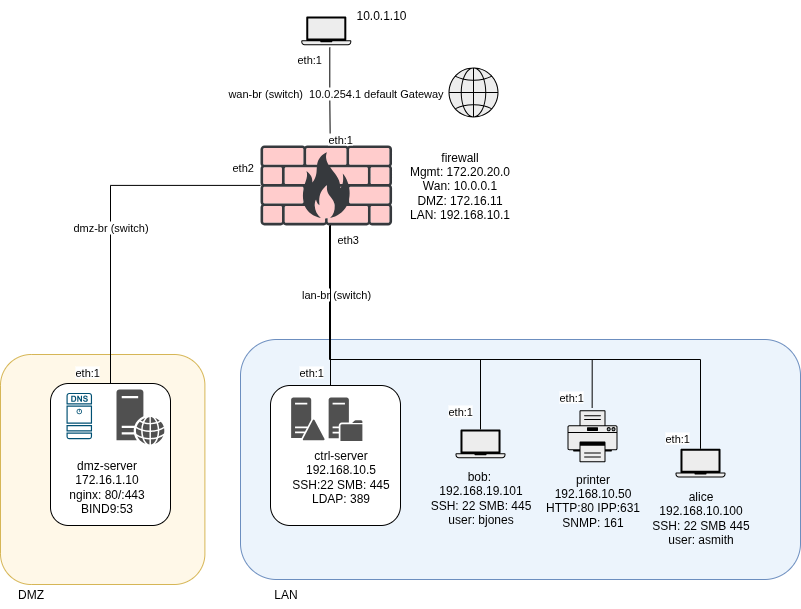
\includegraphics[width=0.8\linewidth]{../assets/diagrams/virtual-environments/virtual-environments.drawio}
	\caption{topology-test-environment}
	\label{fig:virtual-test-environments}
\end{figure}


\subsection{DMZ-Server}\label{subsec:reproducible-test-environment-dmz-server}

To evaluate reconnaissance scenarios, common services must run on endpoints.

\gls{BIND} is a complete implementation of the DNS protocol that can be configured through the \mintinline{bash}|named.conf| file as an authoritative name server and resolver.

In the test lab illustrated in~\ref{fig:virtual-test-environments}, the functionality of the web server and DNS server was combined for simplicity.

During the \gls{DMZ}-server container build process, a setup shell script is executed.

In the first part, the authoritative \gls{BIND} \mintinline{bash}|named.conf| file, DNS options, and master zones for forward and reverse lookups are created.

In the forward zone, domain names map to IP addresses, while in the reverse zone, IP addresses map to domain names~\ref{lst:dmz-server}.

\todo{add filepath and combine with other sections}

\begin{figure}[H]
    \centering
    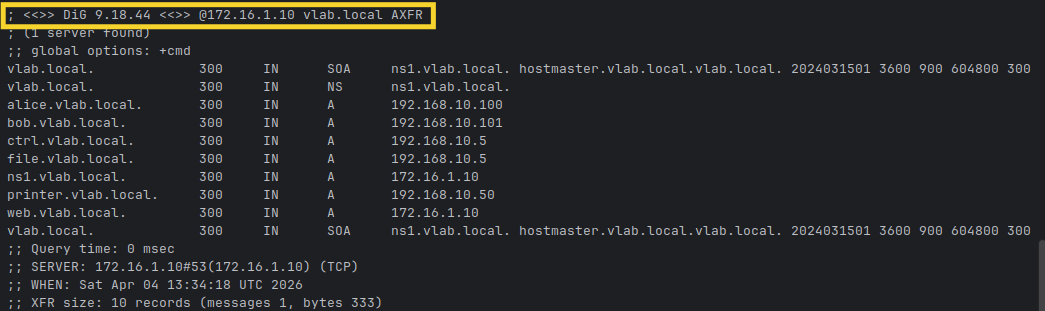
\includegraphics[width=1.0\linewidth]{../assets/screenshots/v-lab/authoritative-zone-transfer-snippet}
    \caption{Authoritative Zone Transfer Snippet}
    \label{fig:authoritative-zone-transfer-snippet}
\end{figure}

The output of a full zone transfer illustrated in figure~\ref{fig:authoritative-zone-transfer-snippet} displays the resolved IP addresses and domain names.
In our test environment, the restriction of \gls{AXFR} requests to only trustworthy IPs is intentionally omitted; the devices are deliberately left unhardened.

In the second part, a minimal \gls{Nginx} web server with HTTP and HTTPS support is created.
Like in real setups, HTTP traffic on port 80 is redirected to HTTPS on port 443.
To provide an artifact for reconnaissance purposes, a file named \mintinline{bash} | {secret.txt} containing sensitive data is placed on the server. |


The LAN zone of the network, consists of 4 devices.


\subsection{Domain Control and File Server}\label{subsec:ctrl-server}

The internal server, reachable at 192.168.10.5, combines the role of domain controller and file server into a single node.

It exposes \gls{SSH} on port 22, \gls{SMB} on ports 139 and 445, and \gls{LDAP} on port 389.

The \gls{LDAP} service is intentionally misconfigured to permit anonymous read access to the entire \mintinline{bash}|dc=lab,dc=local| directory tree, exposing user accounts and group memberships without authentication.

The \gls{SMB} service provides three shares: \mintinline{bash}|public| is readable without credentials, while \mintinline{bash}|finance| and \mintinline{bash}|it| require valid user accounts.

Sensitive files such as payroll exports and budget summaries are placed in the restricted shares as intentional post-exploitation artifacts~\ref{lst:ctrl-server}.

\subsection{Workstations}\label{subsec:workstations}

Two workstations reside on the LAN segment: Alice at 192.168.10.100, assigned to the Finance department, and Bob at 192.168.10.101, assigned to the IT department.

Both nodes expose \gls{SSH} on port 22 and \gls{SMB} on port 445, and both \gls{SSH} banners intentionally disclose the organization name.

On Alice, the home directory of user \mintinline{bash}|asmith| contains a confidential finance report and a drive mapping file that reveals the path to the central file share on the domain server.

On Bob, the home directory of user \mintinline{bash}|bjones| contains a scripts directory with a host inventory that lists all internal IP addresses and their respective roles~\ref{lst:workstations}.

\subsection{Printer}\label{subsec:reproducible-test-environment-printer}

The printer service, reachable at 192.168.10.50, provides two different interfaces.
The first web interface is administrative and is available on port 80.
It shows internal printer metadata, such as device name and contact information.
The printer version is intentionally disclosed in this admin view.
The second interface, a \gls{REST API}, listens on port 631 at the \mintinline{bash}| {/jobs}| endpoint, where it displays a predefined list of print jobs.
All printer requests are logged in \\ \mintinline{bash}|{/var/logs/printer_sim_logs}| inside the container~\ref{lst:printer}.


\subsection{Introduced Vulnerabilities}\label{introduced-vulnerabilities}

For reconnaissance purposes, several vulnerabilities and flaws were introduced, which are partly mentioned in the previous sections and are presented in detail in Listing~\ref{lst:flaws-and-vulnerabilities}. These flaws are necessary to compare the results of the larger and smaller models as well as the implemented vs the AI-enhanced scenarios.
